%\section{Une section}

% remarque : pour qu'un mot se retrouve dans le lexique : \MotDefinition{asymptote horizontale}{} 
\begin{definition}
Un \MotDefinition{triangle isocèle}{} est un triangle qui a deux côtés égaux;

un \MotDefinition{triangle équilatéral}{} est un triangle qui a trois côtés égaux;

un \MotDefinition{triangle rectangle}{} est un triangle qui a deux côtés perpendiculaires.
\end{definition}

\begin{methode*1}[Construire un triangle]

\begin{exemple*1}
Construis un triangle $KLM$ tel que $KL = 6$ cm ; $LM = 5$ cm et $KM = 4,5$ cm :

On trace une figure à \textbf{main levée} :
\begin{center} 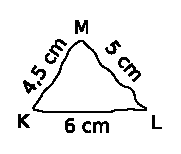
\includegraphics[width=2.3cm]{triangleKML} \end{center}

\begin{tabularx}{\textwidth}{X|X|X}
 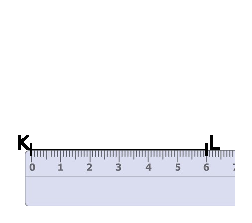
\includegraphics[width=3.1cm]{regleKL} &  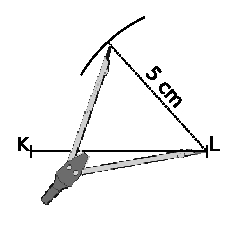
\includegraphics[width=3.1cm]{compasKL} & 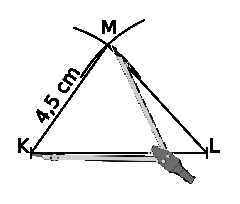
\includegraphics[width=3.1cm]{compasKML} \\ 
 On trace un segment $[KL]$ de longueur 6 cm. & Le point $M$ est à 5 cm du point $L$ : il appartient au cercle de centre $L$ et de rayon 5 cm. & Le point $M$ est à 4,5 cm du point $K$ : il appartient au cercle de centre $K$ et de rayon 4,5 cm. \\
\end{tabularx} \\

\end{exemple*1}

\exercice 
Construis un triangle $VOL$ tel que :

$VO = 4$ cm ; $OL = 6,3$ cm et $LV = 3,8$ cm.

\vspace{2cm}
%\correction

\exercice 
Construis un triangle \textbf{équilatéral} $EAU$ de 45 mm de côté.

\vspace{2cm}
%\correction

\exercice 
Construis le triangle $UNO$ \textbf{isocèle} en $U$ avec :

$UN = 8$ cm et $NO = 3,6$ cm.
%\correction
 
\end{methode*1}

%%%%%%%%%%%%%%%%%%%%%%%%%%%%%%%%%%%%%%%%%%%%%%%%%%

\begin{methode*1}[Construire un triangle rectangle]

\begin{exemple*1}
Construis un triangle $KHI$ rectangle en $K$ tel que $KI = 5$ cm et $HI = 7$ cm : \\[1em]
\begin{tabularx}{\textwidth}{X|X|X|X}
 On trace un segment $[KI]$ de longueur 5 cm (dessins suivants agrandis). & On trace la droite perpendiculaire en $K$ à $(KI)$ et on code l'angle droit. & On trace un arc de cercle de centre $I$ et de rayon 7 cm coupant la perpendiculaire en $H$. & On trace le segment $[HI]$.\\
 
\includegraphics[width=2.2cm]{regle5} & 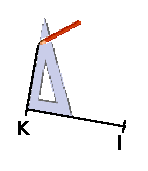
\includegraphics[width=1.8cm]{equerreKI} & 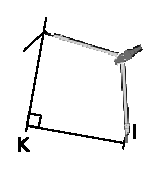
\includegraphics[width=2cm]{compasKI} & 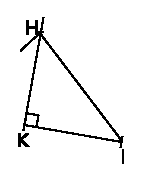
\includegraphics[width=1.8cm]{triangleHKI} \\ 
\end{tabularx} \\

\end{exemple*1}

\exercice 
Construis un triangle $MDR$ rectangle en $D$ tel que :

$MD = 4,2$ cm et $DR = 7,1$ cm. 
\vspace{4cm}
%\correction
 
\exercice
Construis un triangle $ILE$ rectangle en $E$ tel que :

$EL = 6,4$ cm et $LI = 9,3$ cm.
\vspace{2cm}
%\correction
 
\end{methode*1}

%%%%%%%%%%%%%%%%%%%%%%%%%%%%%%%%%%%%%%%%%%%%%%%%%%

\begin{methode*1}[Construire un triangle connaissant un angle et les longueurs \\ de ses côtés adjacents]

 \begin{exemple*1}
Construis un triangle $BAS$ tel que :

$AB = 10,4$ cm ; $BS = 8$ cm et $\widehat{ABS} = 99^\circ$ : \\[1em]
\begin{tabularx}{\textwidth}{X|X|X}
 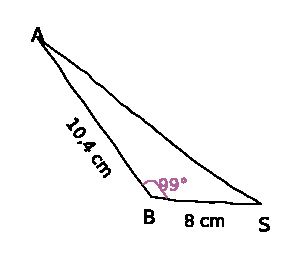
\includegraphics[width=3.3cm]{triangleABS} &  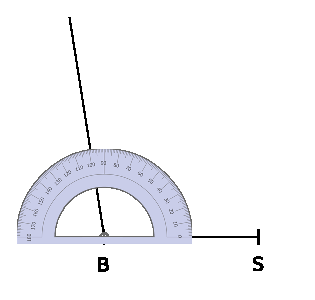
\includegraphics[width=3.5cm]{rapporteurBS} & 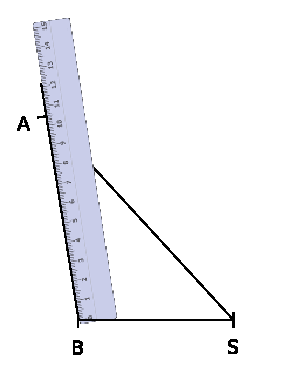
\includegraphics[width=3.6cm]{regleABS} \\ 
 On effectue une figure à main levée en respectant la nature des angles (aigu ou obtus). & On construit un segment $[SB]$ de 8 cm de longueur. On trace un angle mesurant $99^\circ$ de sommet $B$ et de côté $[BS)$. & On place le point $A$ sur le côté de l'angle à 10,4 cm du point $B$. \\
\end{tabularx} \\

\end{exemple*1}

\exercice
Construis un triangle $LET$ tel que :

$\widehat{ETL} = 55^\circ$ ; $ET = 5$ cm et $TL = 4,3$ cm.
\vspace{4cm}
%\correction

\exercice
Construis un triangle $SEL$ tel que :

$SL = 6,4$ cm ; $\widehat{SLE}= 124^\circ$ et $LE = 7,9$ cm.
\vspace{2cm}
%\correction
 
\end{methode*1}


%%%%%%%%%%%%%%%%%%%%%%%%%%%%%%%%%%%%%%%%%%%%%%%%%%

\begin{methode*1}[Construire un triangle connaissant deux angles et la longueur \\ de leur côté commun]

 \begin{exemple*1}
Construis le triangle $GAZ$ tel que :

$AZ = 11,2$ cm ; $\widehat{GAZ} = 100^\circ$ et $\widehat{AZG} = 31^\circ$. \\[1em]
\begin{tabularx}{\textwidth}{X|X|X}
 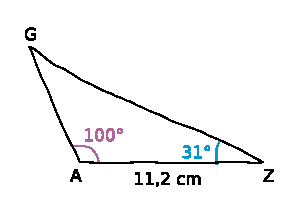
\includegraphics[width=3.3cm]{triangleGAZ} &  \includegraphics[width=3.0cm]{rapporteurAZ} & \includegraphics[width=3.0cm]{rapporteurGAZ} \\ 
 On effectue une figure à main levée en respectant la nature des angles (aigu ou obtus). & On trace un segment $[AZ]$ de longueur 11,2 cm. On construit un angle de sommet $A$, de côté $[AZ)$ et mesurant $100^\circ$. & On construit un angle de sommet $Z$, de côté $[ZA)$ et mesurant $31^\circ$. Les côtés des deux angles se coupent au point $G$. \\
\end{tabularx} \\

\end{exemple*1}

\exercice
Construis le triangle $SUD$ tel que :

$UD = 6$ cm ; $\widehat{SUD} = 65^\circ$ ; $\widehat{SDU} = 36^\circ$.
\vspace{4cm}
%\correction

\exercice
Construis le triangle $EST$ tel que :

$ET = 4,6$ cm ; $\widehat{SET} = 93^\circ$ et $\widehat{ETS} = 34^\circ$.
\vspace{2cm}
%\correction
 
\end{methode*1}



\newpage

%%%%%%%%%%%%%%%%%%%%%%%%%%%%%%%%%%%%%%%%%%%%%%%%%%%%%%%%%%%%%%%%%%%%%%%%%%%%%%%%%
%Médiatrice

 \begin{aconnaitre}
Les médiatrices des trois côtés d'un triangle sont \MotDefinition{concourantes}{}.

Leur point d'intersection est le centre du \MotDefinition{cercle circonscrit}{} au triangle. Ce cercle passe par les trois sommets du triangle.
\end{aconnaitre}

 \vspace{2em}
 
 \begin{methode*1}[Construire le cercle circonscrit à un triangle]
 
\begin{remarque}
Il suffit de tracer les médiatrices de deux côtés pour déterminer le centre du cercle circonscrit.
 \end{remarque}
 
 \begin{exemple*1}
Trace le cercle circonscrit au triangle $PAF$ :
 \begin{tabularx}{\textwidth}{X|X|X}
 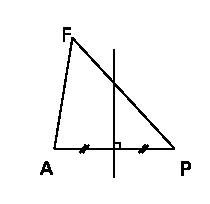
\includegraphics[width=3.2cm]{triangleFAP} &  \includegraphics[width=3.2cm]{triangleFAOP} & 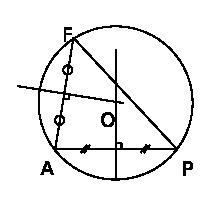
\includegraphics[width=3.2cm]{triangle_cercleFAOP} \\ 
 On construit la médiatrice du segment $[AP]$. & On construit la médiatrice du segment $[FA]$. Soit $O$ le point d'intersection des deux médiatrices. & Le cercle circonscrit est le cercle de centre $O$ et de rayon $OA$ (ou $OF$ ou $OP$). \\
\end{tabularx} \\

\end{exemple*1}

\exercice
Construis le triangle $FEU$ tel que :

$FE = 6$ cm ; $EU = 3,7$ cm et $UF = 3,5$ cm. Trace le cercle circonscrit au triangle $FEU$.
\vspace{4cm}
%\correction

\exercice
Construis le triangle $EAU$ et son cercle circonscrit sachant que : $EA = 6,1$ cm ; $AU = 3$ cm et $UE = 4,9$ cm.

\vspace{2cm}
%\correction

\end{methode*1}



%%%%%%%%%%%%%%%%%%%%%%%%%%%%%%%%%%%%%%%%%%%%%%%%%%
%Médiane


\newpage

\begin{definition}
Dans un triangle, une \MotDefinition{médiane}{} est une droite qui passe par un sommet du triangle et par le milieu du côté opposé à ce sommet.

Les trois médianes d'un triangle sont concourantes en un point, noté G, et appelé \MotDefinition{centre de gravité}{} du triangle.
\end{definition}

\vspace{2em}

\begin{methode*1}[Construire le centre de gravité d'un triangle]

\begin{remarque}
Puisque les trois médianes sont concourantes, il suffit d'en tracer deux pour déterminer le centre de gravité.
 \end{remarque}

 \begin{exemple*1}
 Trace la centre de gravité du triangle $ABC$ :
 \begin{tabularx}{\textwidth}{X|X|X}
 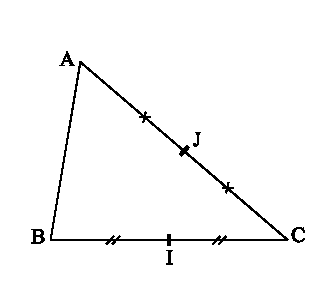
\includegraphics[width=3.2cm]{CentreGravite1} &  \includegraphics[width=3.2cm]{CentreGravite2} & 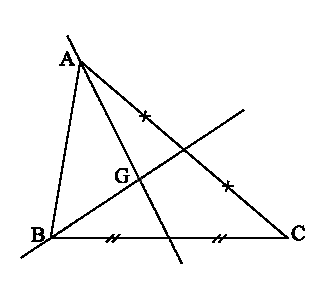
\includegraphics[width=3.1cm]{CentreGravite3} \\ 
 On trace le milieu de deux des côtés (ici I et J). & On trace les médianes passant par ces deux milieux & Le centre de gravité G est le point d'intertection des médianes. \\
\end{tabularx} \\

\end{exemple*1}

 
\exercice
Construis le triangle $CLE$ tel que 
$CL = 4,5$ cm ; $CE = 5,2$ cm et $\widehat{CLE} = 78^\circ$ puis trace son centre de gravité.
%\correction


\end{methode*1}


%%%%%%%%%%%%%%%%%%%%%%%%%%%%%%%%%%%%%%%%%%%%%%%%%%
%Hauteurs

\newpage

\begin{definition}
Dans un triangle, une \MotDefinition{hauteur}{} est une droite qui passe par un sommet du triangle et qui est perpendiculaire au côté opposé à ce sommet.

Les trois hauteurs d'un triangle sont concourantes en un point, noté H, et appelé \MotDefinition{orthocentre}{} du triangle.
\end{definition}

\vspace{2em}

\begin{methode*1}[Construire les hauteurs d'un triangle]

 \begin{exemple*1}
 Trace la hauteur relative au côté $[BR]$ :
 \begin{tabularx}{\textwidth}{X|X|X}
 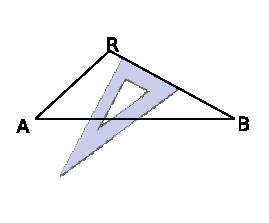
\includegraphics[width=3.2cm]{triangleARB_1} &  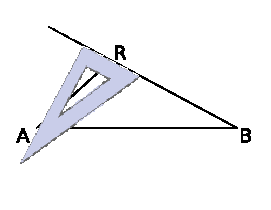
\includegraphics[width=3.2cm]{triangleARB_2} & 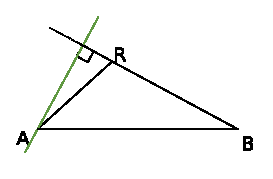
\includegraphics[width=3.1cm]{triangleARB_3} \\ 
 On positionne l'équerre perpendiculairement au côté $[BR]$. & On fait glisser l'équerre jusqu'au point $A$. Il faut parfois prolonger le côté $[BR]$. & La hauteur relative au côté $[BR]$ est la droite perpendiculaire au côté $[BR]$ et passant par $A$. \\
\end{tabularx} \\

\end{exemple*1}

\begin{remarque}
On dit aussi «hauteur issue du sommet $A$» pour nommer la hauteur relative au côté $[BR]$.
 \end{remarque}
 
\exercice
Construis le triangle $CAR$ tel que 
$CA = 4,6$ cm ; $AR = 4,3$ cm et $\widehat{CAR} = 102^\circ$ puis trace la hauteur issue de $R$ et celle issue de $C$.
\vspace{2cm}
%\correction
     
\exercice
Construis un triangle $TAX$ tel que 

$TA = 6,3$ cm ; $\widehat{TAX} = 57^\circ$ et $\widehat{ATX} = 63^\circ$ puis trace ses hauteurs.
\vspace{2cm}
%\correction

\exercice
Construis un triangle $BUS$ tel que :

$BU = 6,4$ cm ; $US = 4,8$ cm et $BS = 8$ cm. Trace les trois hauteurs de ce triangle.
%\correction

\end{methode*1}



%%%%%%%%%%%%%%%%%%%%%%%%%%%%%%%%%%%%%%%%%%%%%%%%%%
%Bissectrices

 \newpage
 
 \begin{aconnaitre}
Les trois bissectrices des angles d'un triangle sont concourantes. 

Leur point d'intersection est le \MotDefinition{centre du cercle inscrit}{} dans le triangle. Ce cercle est tangent aux trois côtés du triangle.
 \end{aconnaitre}
 
 \vspace{2em}
 
 \begin{methode*1}[Centre du cercle inscrit dans un triangle]
 
 \begin{remarque}
Il suffit de tracer les bissectrices de deux angles pour déterminer le centre du cercle inscrit.
 \end{remarque}
 
 \begin{exemple*1}
 Construis un triangle $MER$ et son cercle inscrit de centre $O$ :
 \begin{tabularx}{\textwidth}{X|X|X}
 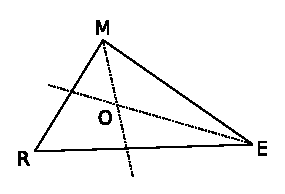
\includegraphics[width=3.2cm]{triangleMRE} &  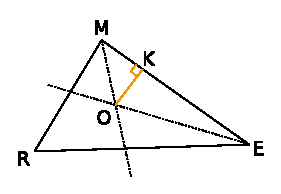
\includegraphics[width=3.2cm]{triangleMREK} & 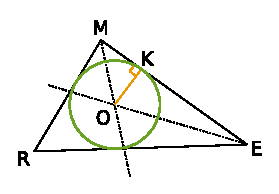
\includegraphics[width=3.2cm]{triangle_cercleMREK} \\ 
 On trace les bissectrices de deux des trois angles du triangle $MER$. Elles se coupent en $O$, le centre du cercle inscrit. & On trace la perpendiculaire à $(ME)$ passant par le point $O$. Elle coupe $[ME]$ en $K$. On obtient ainsi un rayon $[OK]$ du cercle inscrit dans le triangle $MER$. & On trace le cercle de centre $O$ passant par $K$. \\
 \end{tabularx} \\

\end{exemple*1}
 
 \exercice
Construis un triangle $RAS$ tel que 

$RA = 7$ cm ; $AS = 8$ cm et $RS = 9$ cm puis son cercle inscrit.
%\correction
 
 \end{methode*1}

